\documentclass[english,11pt]{beamer}

\DeclareMathOperator{\Cov}{Cov}
\DeclareMathOperator{\Var}{Var}
\DeclareMathOperator{\E}{\mathbb{E}}
\DeclareMathOperator{\Proba}{\mathbb{P}}

\newcommand{\Covb}[2]{\ensuremath{\Cov\!\left[#1,#2\right]}}
\newcommand{\Eb}[1]{\ensuremath{\E\!\left[#1\right]}}
\newcommand{\Pb}[1]{\ensuremath{\Proba\!\left[#1\right]}}
\newcommand{\Varb}[1]{\ensuremath{\Var\!\left[#1\right]}}

% norm
\newcommand{\norm}[1]{\| #1 \|}

\newcommand{\indep}{\rotatebox[origin=c]{90}{$\models$}}





\usepackage{mathptmx,amsmath,amssymb,graphicx,bibentry,bbm,babel,ragged2e}

\makeatletter

\newcommand{\noun}[1]{\textsc{#1}}
\newcommand{\jitem}[1]{\item \begin{justify} #1 \end{justify} \vfill{}}
\newcommand{\sframe}[2]{\frame{\frametitle{#1} #2}}

\newenvironment{centercolumns}{\begin{columns}[c]}{\end{columns}}
%\newenvironment{jitem}{\begin{justify}\begin{itemize}}{\end{itemize}\end{justify}}

\usetheme{Warsaw}
\setbeamertemplate{footline}[text line]{}
\setbeamertemplate{headline}{}
\setbeamercolor{structure}{fg=purple!50!blue, bg=purple!50!blue}

\setbeamersize{text margin left=15pt,text margin right=15pt}

\setbeamercovered{transparent}


\@ifundefined{showcaptionsetup}{}{%
 \PassOptionsToPackage{caption=false}{subfig}}
\usepackage{subfig}

\usepackage[utf8]{inputenc}
\usepackage[T1]{fontenc}

\usepackage{multirow}

\usepackage{pifont}
%\newcommand{\cmark}{\textcolor{green}\ding{51}}
%\newcommand{\xmark}{\textcolor{red}\ding{55}}
\newcommand{\cmark}{\ding{51}}
\newcommand{\xmark}{\ding{55}}

\makeatother



\title{Generating urban morphologies at large scales}
\author{Juste Raimbault$^{1,2,3,*}$ and Julien Perret$^{1,4}$}
\institute{$^1$UPS CNRS 3611 ISC-PIF\\
$^2$CASA, UCL\\
$^3$UMR CNRS 8504 G{\'e}ographie-cit{\'e}s\\
$^4$Univ. Paris-Est, LaSTIG STRUDEL, IGN, ENSG\\
\medskip
* juste.raimbault@polytechnique.edu
}
\date{Artificial Life 2019\\\bigskip
Monday 29th July, 2019}

\begin{document}



\begin{frame}%[plain]
	\titlepage
\end{frame}
%\addtocounter{framenumber}{-1}



\sframe{Morphogenesis of Urban Systems}{

% + Urban science building !

\begin{center}
	\includegraphics[width=\textwidth]{figuresslides/helix.png}	
\end{center}

\medskip

``\textit{new innovation community, sustainable urban development, flourishing city, urban regeneration}''

\medskip

$\rightarrow$ Are cities alive? Which morphogenetic processes?

% TODO idea next year : all feature of urban systems making them candidate for alife ? (more than thought :cf innovatino etc. we come back to coevol and morphogenesis ? possibly - a bit far ?)

}


\sframe{Urban Systems and Artificial Life}{

\begin{columns}

	\begin{column}{0.5\textwidth}
	
	\vspace{-0.5cm}
	
	\begin{center}
	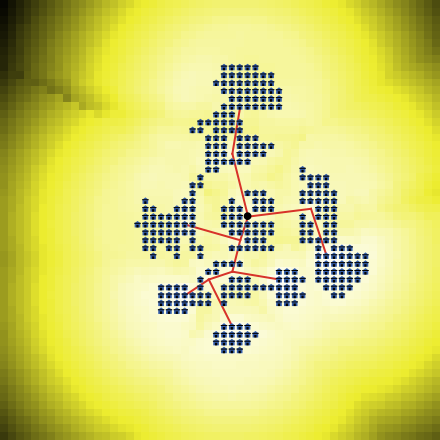
\includegraphics[width=0.8\textwidth]{figuresslides/intro_RBD_lattice.png}
	\end{center}
	
	\medskip
	
	\footnotesize
\textit{Hybrid urban morphogenesis with simple rules for urban sprawl and road network evolution}
	
	\medskip
	
	\tiny

	Raimbault, J., Banos, A., & Doursat, R. (2014). A Hybrid Network/Grid Model of Urban Morphogenesis and Optimization. In 4th International Conference on Complex Systems and Applications (pp. 51-60).	
	
	\nocite{raimbault2014hybrid}

	\end{column}
	\vrule{}
	\begin{column}{0.5\textwidth}
	
	\vspace{-0.5cm}
	\begin{center}
	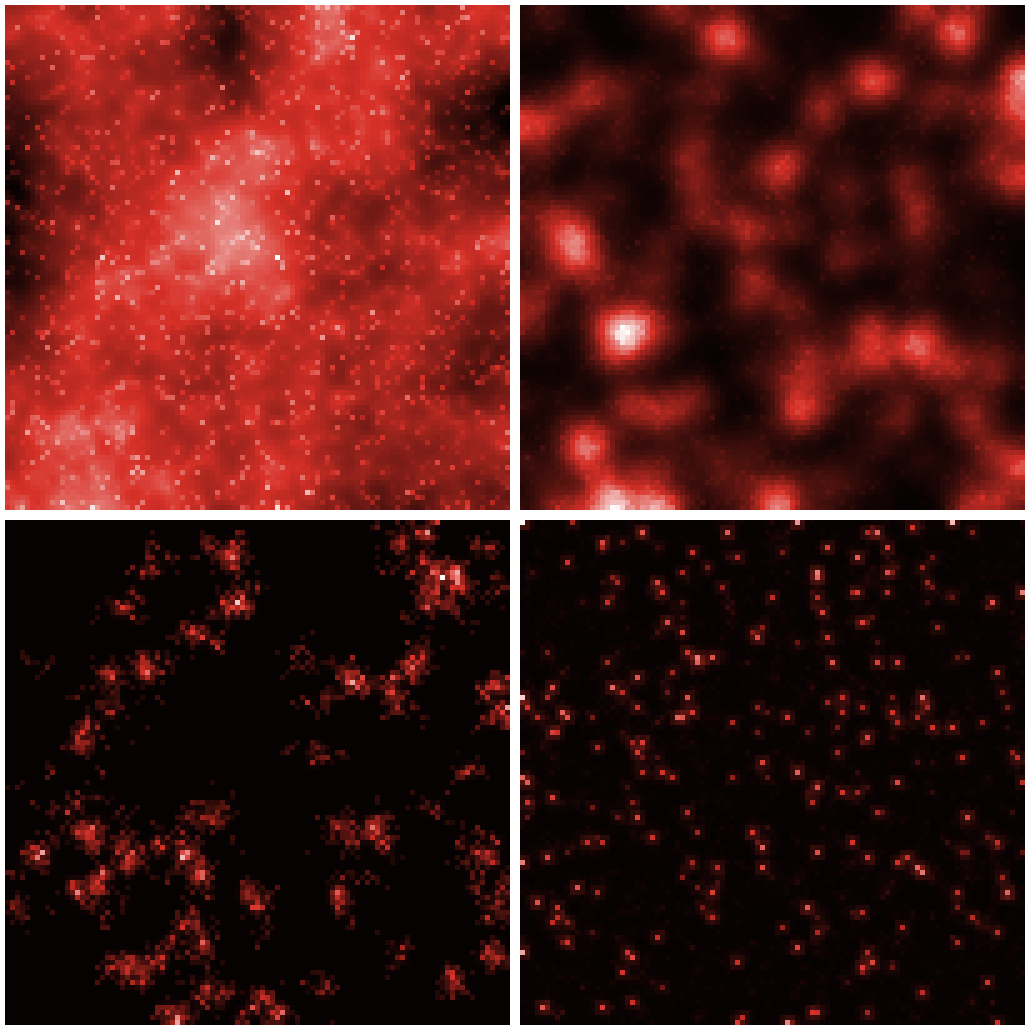
\includegraphics[width=0.8\textwidth]{figuresslides/density_Fig2}
	\end{center}
	
	\medskip
	\footnotesize
	
	\textit{Reaction-diffusion processes to reproduce territorial settlements at an intermediate scale}
	
	\medskip
	
	\tiny
	
Raimbault, J. (2018). Calibration of a density-based model of urban morphogenesis. PloS one, 13(9), e0203516.

\nocite{raimbault2018calibration}

\smallskip

Raimbault, J. (2019). An urban morphogenesis model capturing interactions between networks and territories. In The Mathematics of Urban Morphology (pp. 383-409). Birkhäuser, Cham.

\nocite{raimbault2019urban}
	

	\end{column}

\end{columns}

}


\sframe{Urban Systems and Artificial Life}{

\begin{columns}

	\begin{column}{0.5\textwidth}

\begin{center}
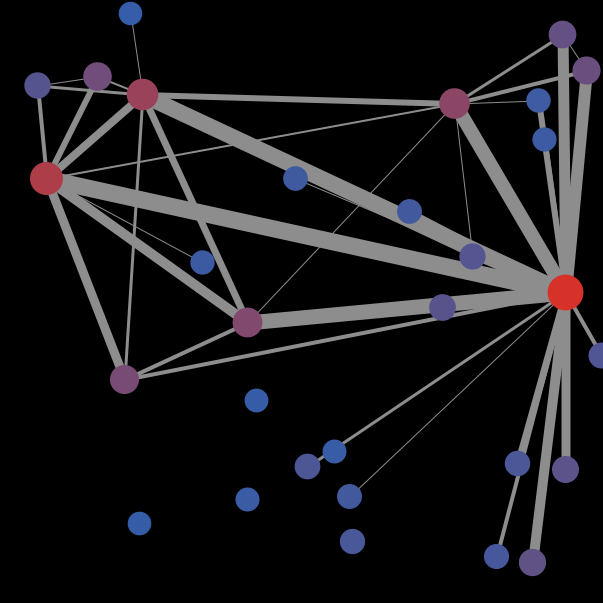
\includegraphics[height=0.47\textheight]{figuresslides/macrocoevol_example_virtual_0_tf.png}
\end{center}

	\medskip

	\footnotesize
	\textit{Cities-network co-evolution model explored on synthetic systems of cities} 

\medskip

\tiny

	Raimbault, J. (2019). Modeling the co-evolution of cities and networks. Forthcoming in Handbook of Cities and Networks, Rozenblat C., Niel Z., eds.

	\nocite{raimbault2019modeling}
	

	\end{column}
	\vrule{}
	\begin{column}{0.5\textwidth}

	\begin{center}
		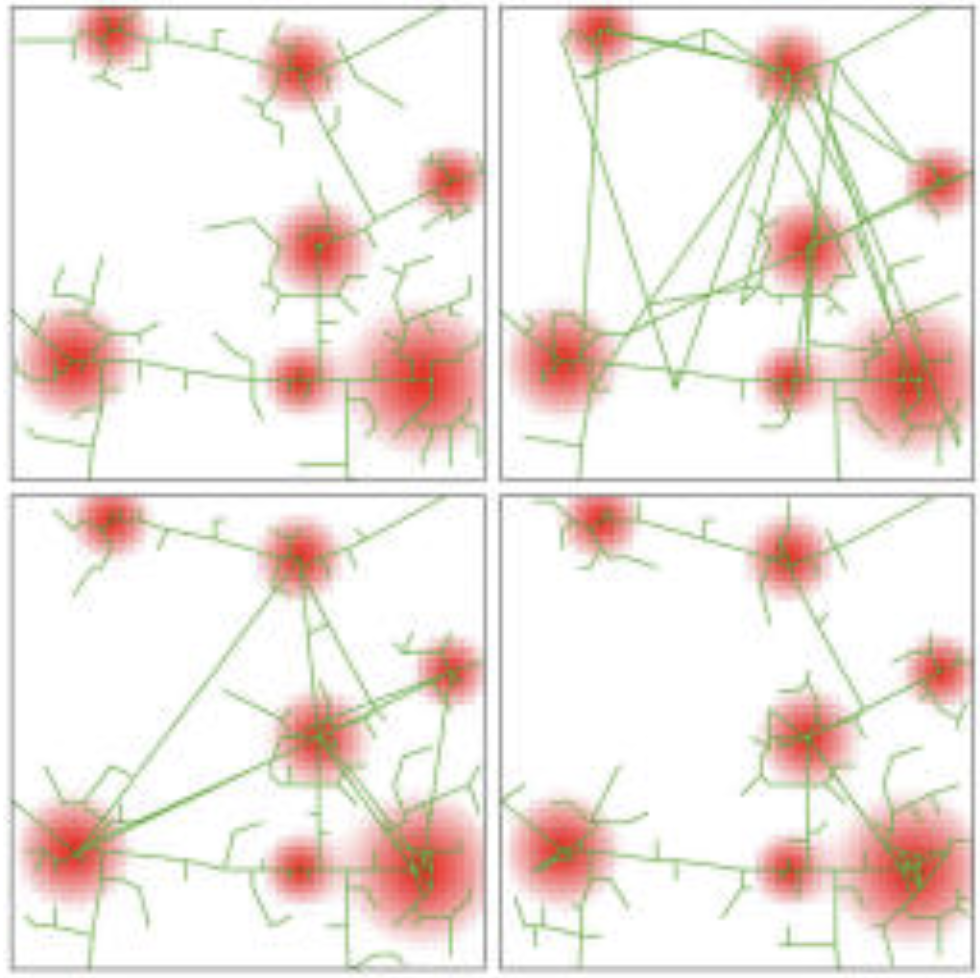
\includegraphics[width=0.8\textwidth]{figuresslides/nwmorphogenesis.png}
	\end{center}

	\medskip

	\footnotesize

	\textit{Complementary heuristics to reproduce topological properties of transportation networks}	

 	\medskip
	\tiny

	Raimbault, J. (2018). Multi-modeling the morphogenesis of transportation networks. In Artificial Life 2018 Conference Proceedings (pp. 382-383).

	\nocite{raimbault2018multi}

	\end{column}

\end{columns}	

}





\sframe{Urban form from the bottom up}{

%systematic comparison of simple processual generators
%	\item introduction of morphological indicators
%	\item calibration on sampled layouts from OpenStreetMap

$\rightarrow$ Emergence of the urban form from local processes

\medskip

$\rightarrow$ Particularity of large geographical scales (building layout morphogenesis)

\medskip

$\rightarrow$ Quantitative indicators to measure urban form


\bigskip
\bigskip

\textbf{Research objective: } 

\medskip

\textit{Introduce simple generative models for urban configurations at the district scale; introduce a set of indicators to classify model outputs; investigate the potentiality of generative models to produce existing configurations.}

}






\sframe{Generating building layouts}{

Complementary heuristics:

\medskip

\begin{itemize}
	\item random building blocks (modern urbanism)
	\item thresholded kernel mixture (hybrid configurations / preferential attachment for population)
	\item percolation of roads through a compact urban core (transportation flows)
\end{itemize}

\bigskip


\begin{columns}
	\begin{column}{0.31\textwidth}
		
		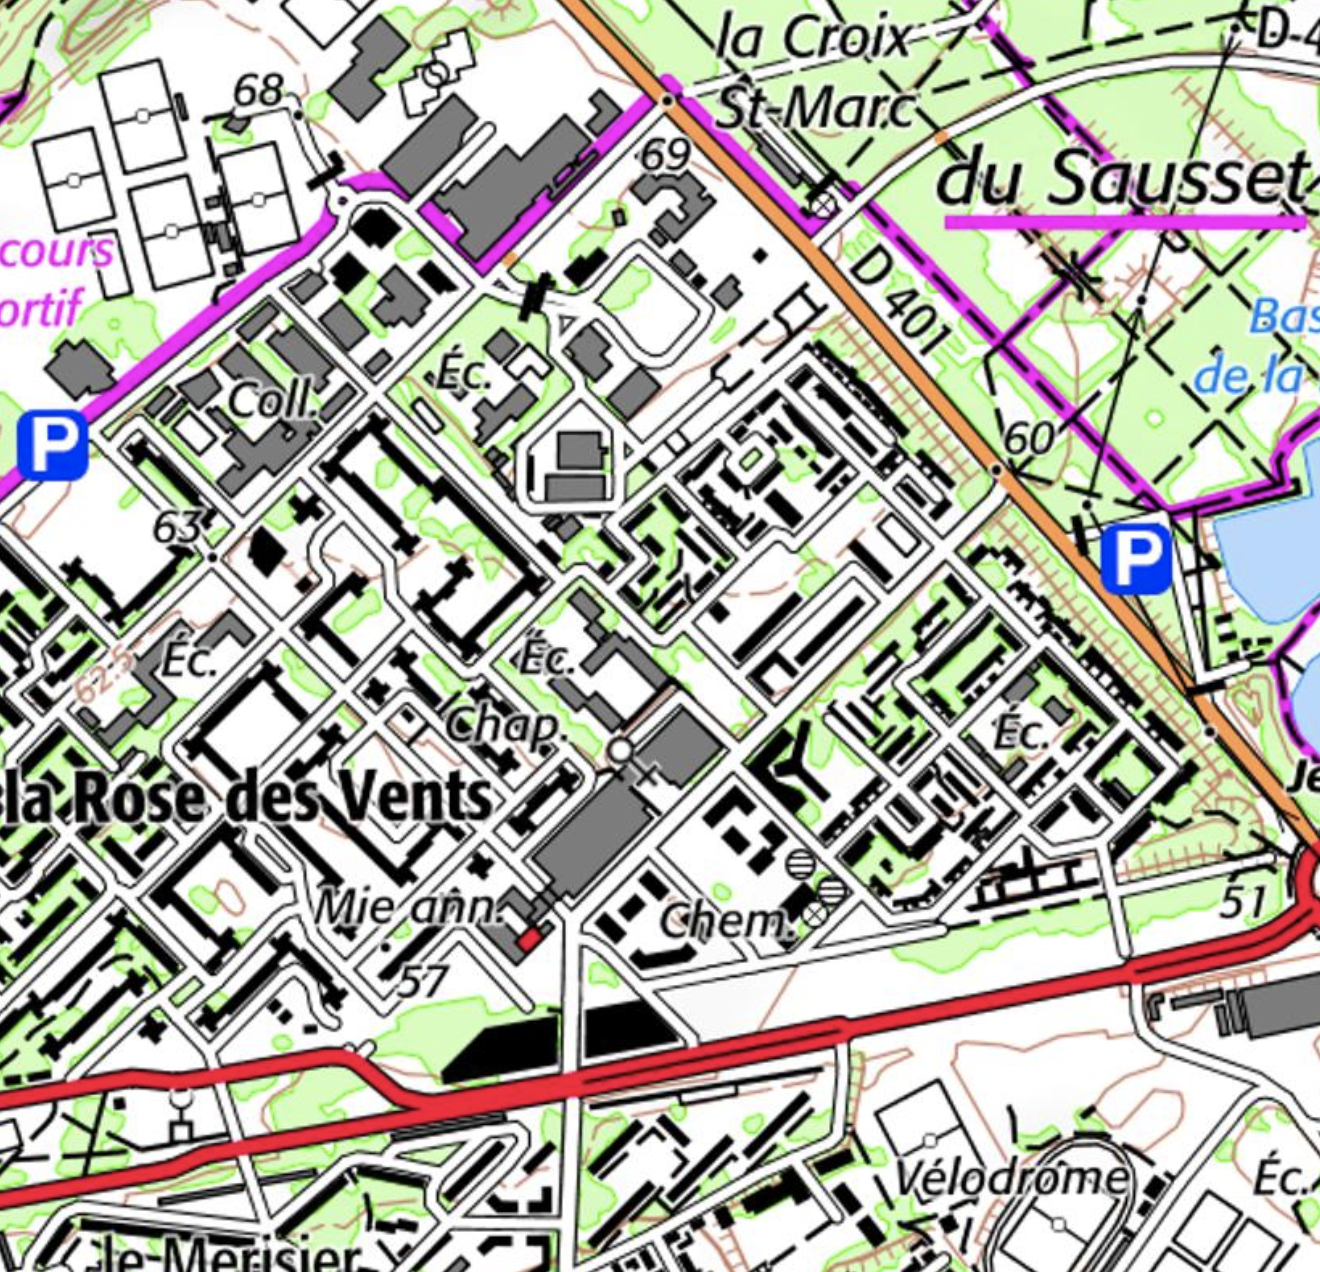
\includegraphics[width=\textwidth]{figuresslides/morpho_aulnay.png}
	
	\end{column}
	\vrule{}
	\begin{column}{0.33\textwidth}
	
		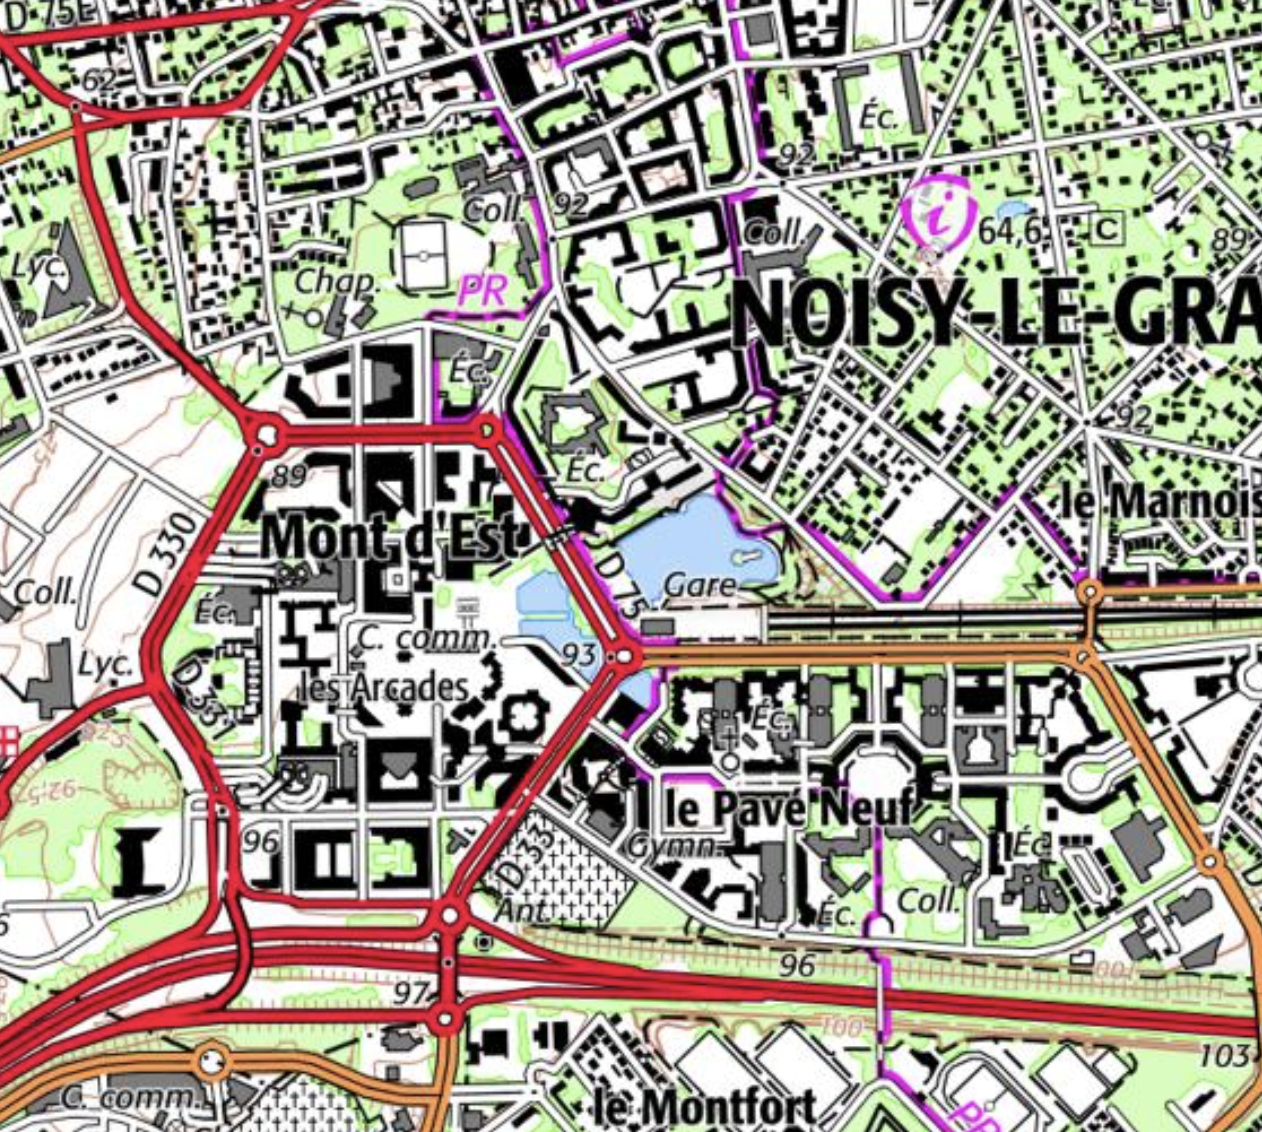
\includegraphics[width=\textwidth]{figuresslides/morpho_montdest.png}
		
	\end{column}
	\vrule{}
	\begin{column}{0.31\textwidth}
		
		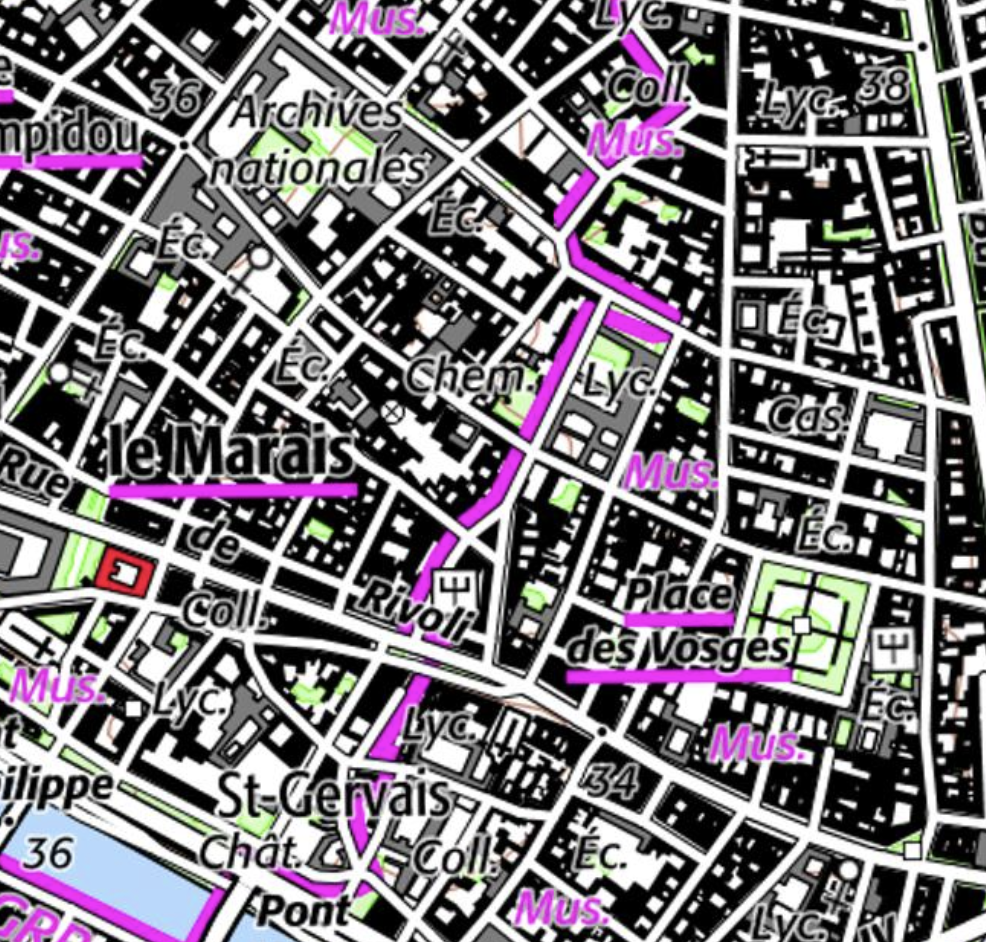
\includegraphics[width=\textwidth]{figuresslides/morpho_marais.png}
	
	\end{column}
\end{columns}
}

}


\sframe{Quantifying urban form}{

% Simple descriptive indicators considered are (i) the total building density $A = \frac{1}{N}\cdot \sum_i s_i$; (ii) the number of buildings given by the number of connected components of $B$; (iii) the average building area, i.e. the average size of $B$ connected components; (iv) Moran index capturing spatial autocorrelation (see \cite{raimbault2018calibration} for its definition in a similar setting), with a simple inverse distance weight function; (v) average distance between non-empty points (which also captures a level of concentration).
% We also use indicators computed with the underlying networks: the average detour computed in the free space network $\bar{B}$, computed by randomly sampling 50 pairs of points in a connected component of $\bar{B}$ and computing the ratio between the network distance and the euclidian distance $d_{\bar{B}}/d_E$. This measures captures in a way the sinuosity of streets from a mobility viewpoint. We also consider the average size of open connected areas as the average size of the connected components of $\bar{B}$.
% steps for dilation + steps for erosion


Urban form indicators for building layouts:

\medskip

\begin{itemize}
	\item Density, number of buildings, average area
	\item Moran index (spatial autocorrelation) and average distance on rasterized representation
	\item Average detour in the free space
	\item Mathematical morphology indicators (steps for erosion and dilation) \cite{serra1983image}
\end{itemize}


}


\sframe{Generators}{

\vspace{-0.3cm}
\begin{center}
	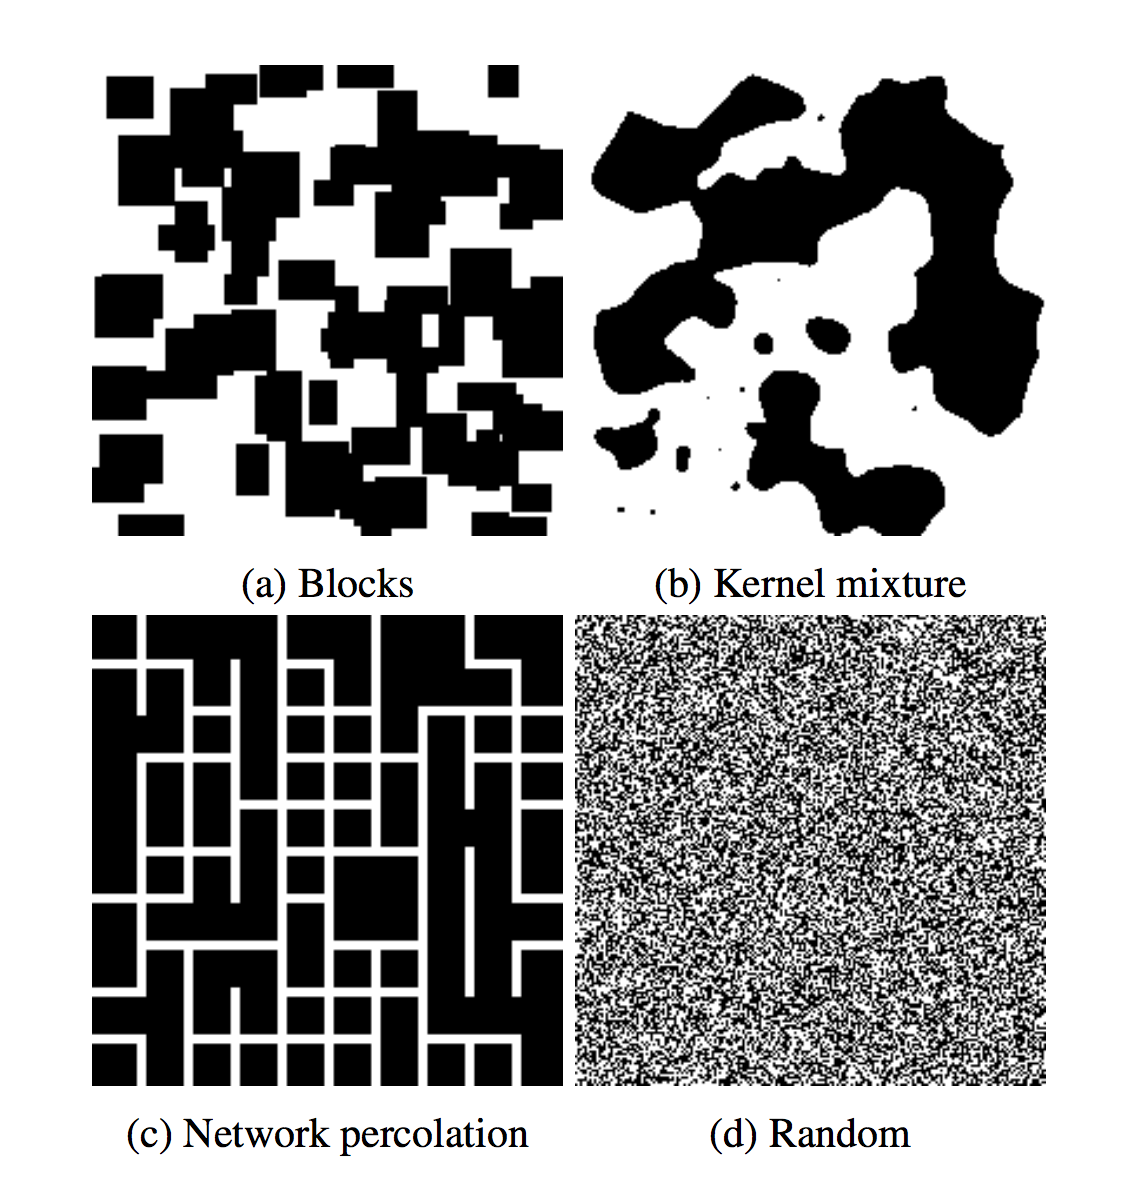
\includegraphics[height=0.85\textheight]{figuresslides/spatialsens_examplegenerators.png}
\end{center}

\vspace{-0.2cm}

\textit{Examples of urban forms for each generator (3 parameters each)}


}

\sframe{Real configurations}{

\vspace{-0.3cm}
\begin{center}
	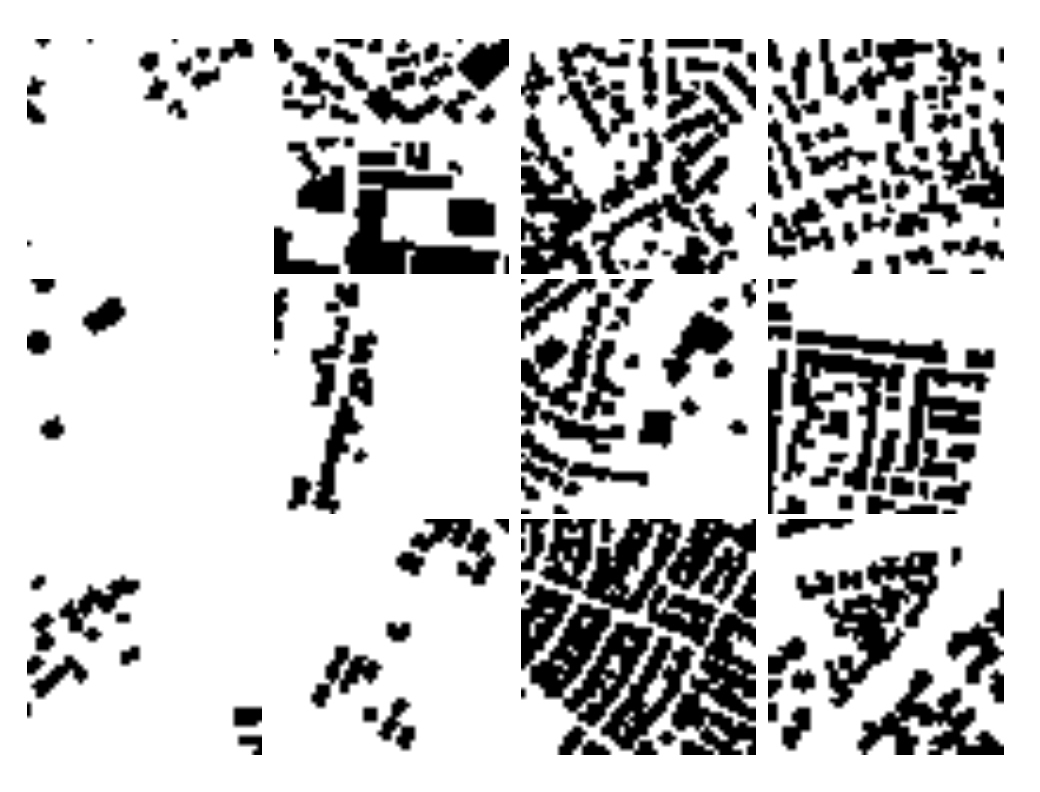
\includegraphics[height=0.82\textheight]{figuresslides/spatialsens_exampleosm.png}
\end{center}

\vspace{-0.2cm}

\footnotesize

\textit{Sampled districts from OpenStreetMap (72,000 real district sampled accross European functional urban areas \cite{bretagnolle2019following})}

}


\sframe{Classification of urban forms}{

\vspace{-0.3cm}
\begin{center}
   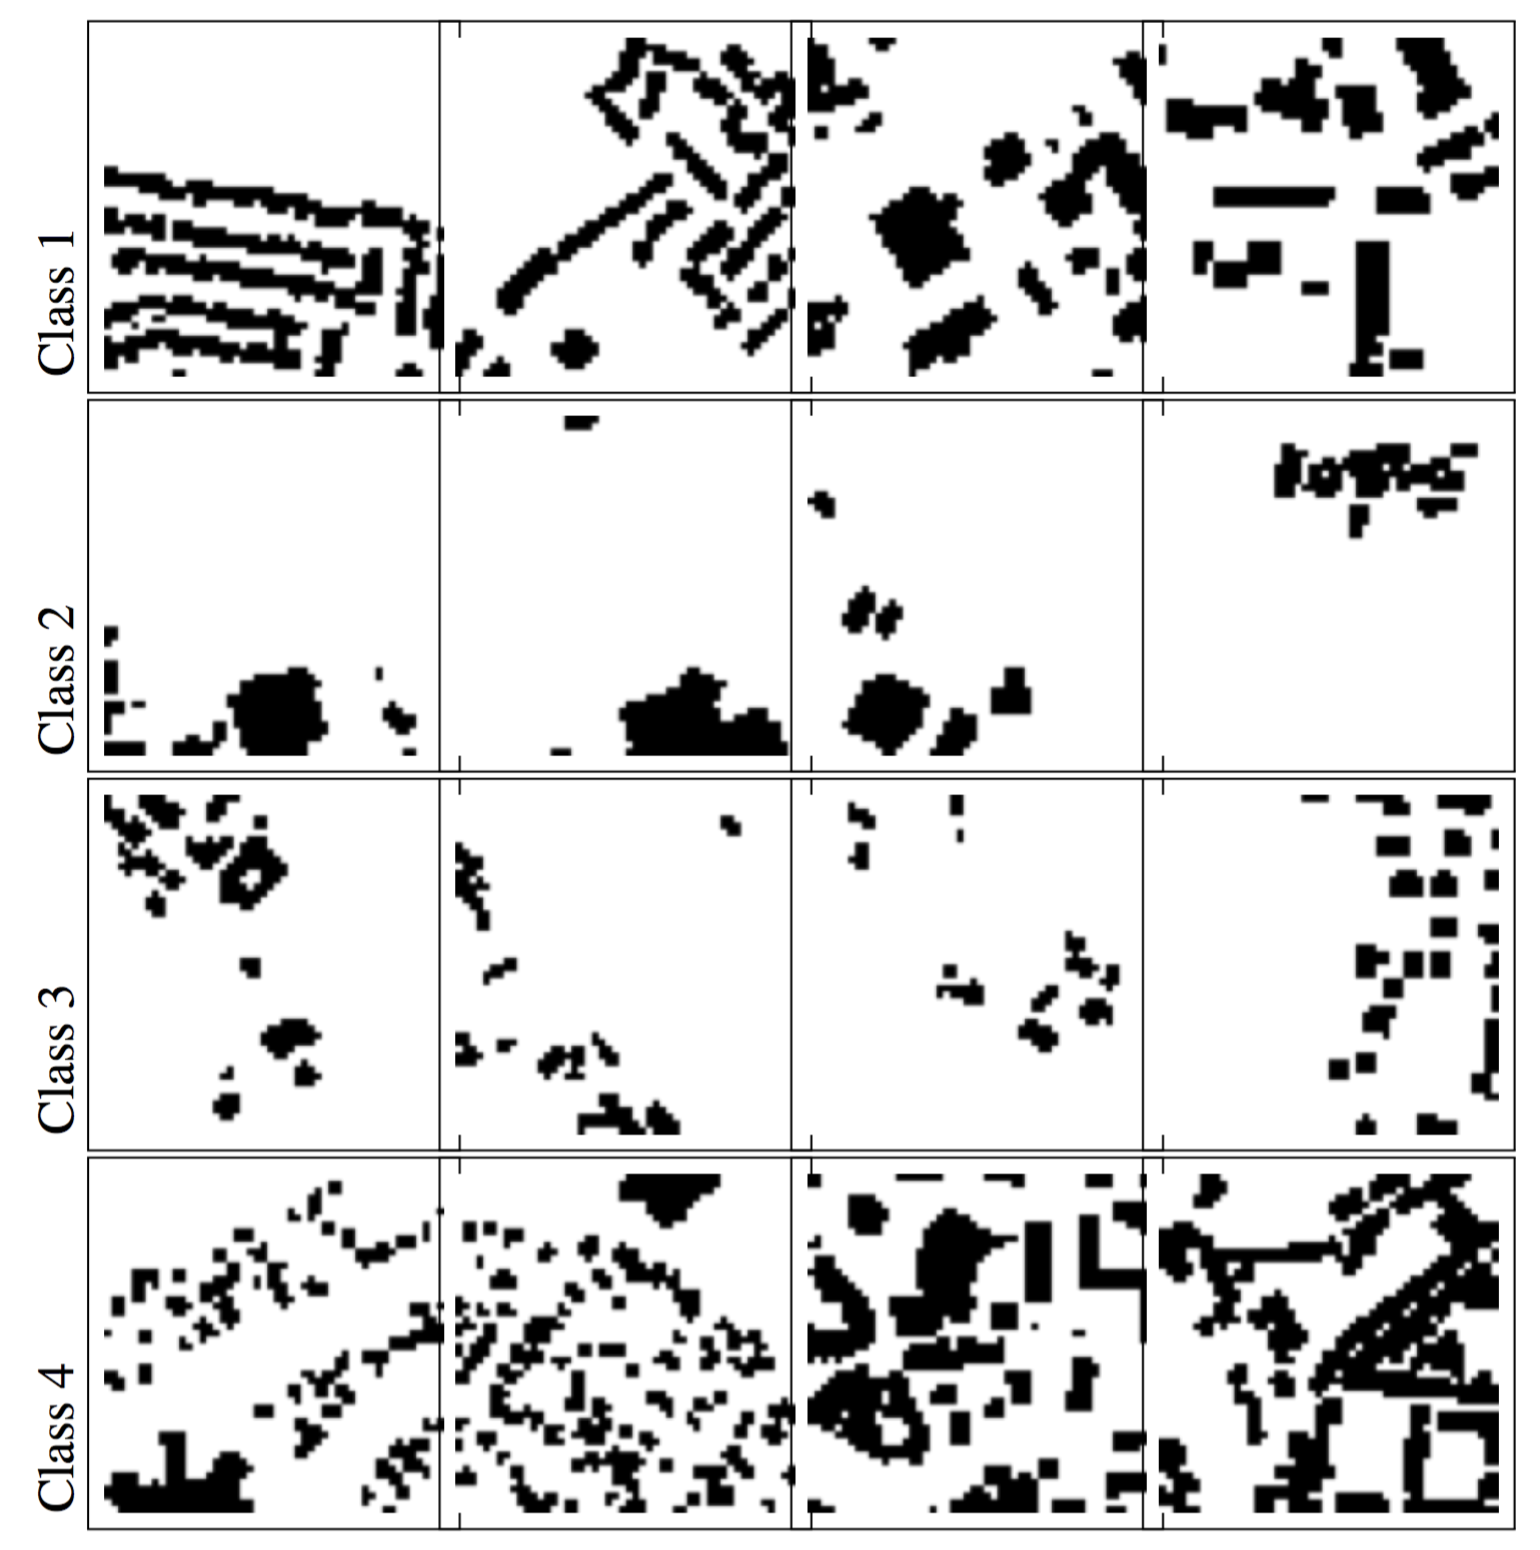
\includegraphics[height=0.82\textheight]{figuresslides/spatialsens_osm_classification.png}
\end{center}

\vspace{-0.2cm}

\footnotesize

\textit{Unsupervised classification of real morphologies (effective dimension: 85.9\% of variance at second PC)}

}



\sframe{Model calibration tool}{

Models explored and calibrated with the OpenMOLE software~\cite{reuillon2013openmole}

\centering

\bigskip


\includegraphics[height=0.35\textheight]{figuresslides/openmole.png}

\bigskip

\raggedright\justify

\footnotesize \textit{OpenMOLE: (i) embeds any model as a black box; (ii) provides transparent access to main High Performance Computing environments; (iii) and to model exploration and calibration methods (sensitivity analysis, Design of Experiments, Genetic Algorithm calibration, Diversity Search).}

\medskip

\textbf{Free and Open Source, download at} \url{https://openmole.org/}

}




\sframe{Calibrated forms}{

\begin{center}
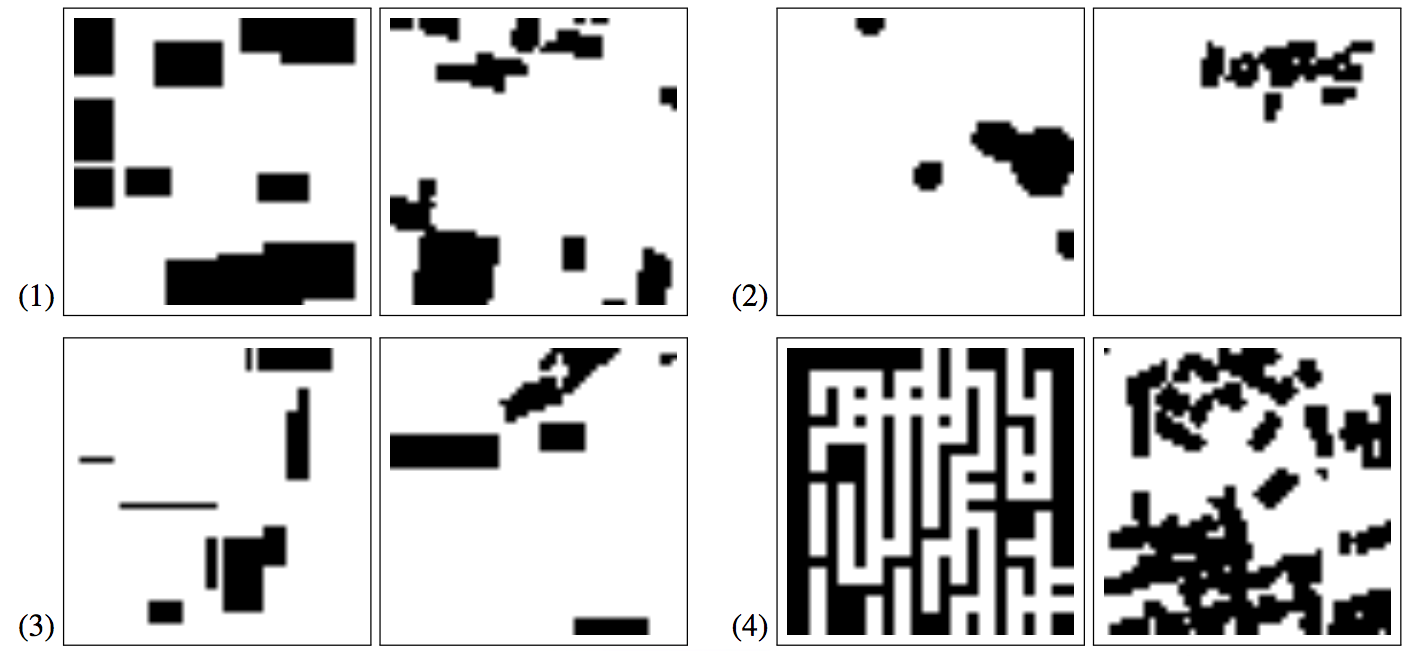
\includegraphics[width=\textwidth]{figuresslides/spatialsens_calib.png}
\end{center}

\smallskip

\textit{Example of close real and simulated configurations, after running the model for 10,000 random parameter points (LHS) for each generator, with 100 stochastic repetitions each}

}


\sframe{Comparison of point clouds}{

\vspace{-0.2cm}
\begin{center}
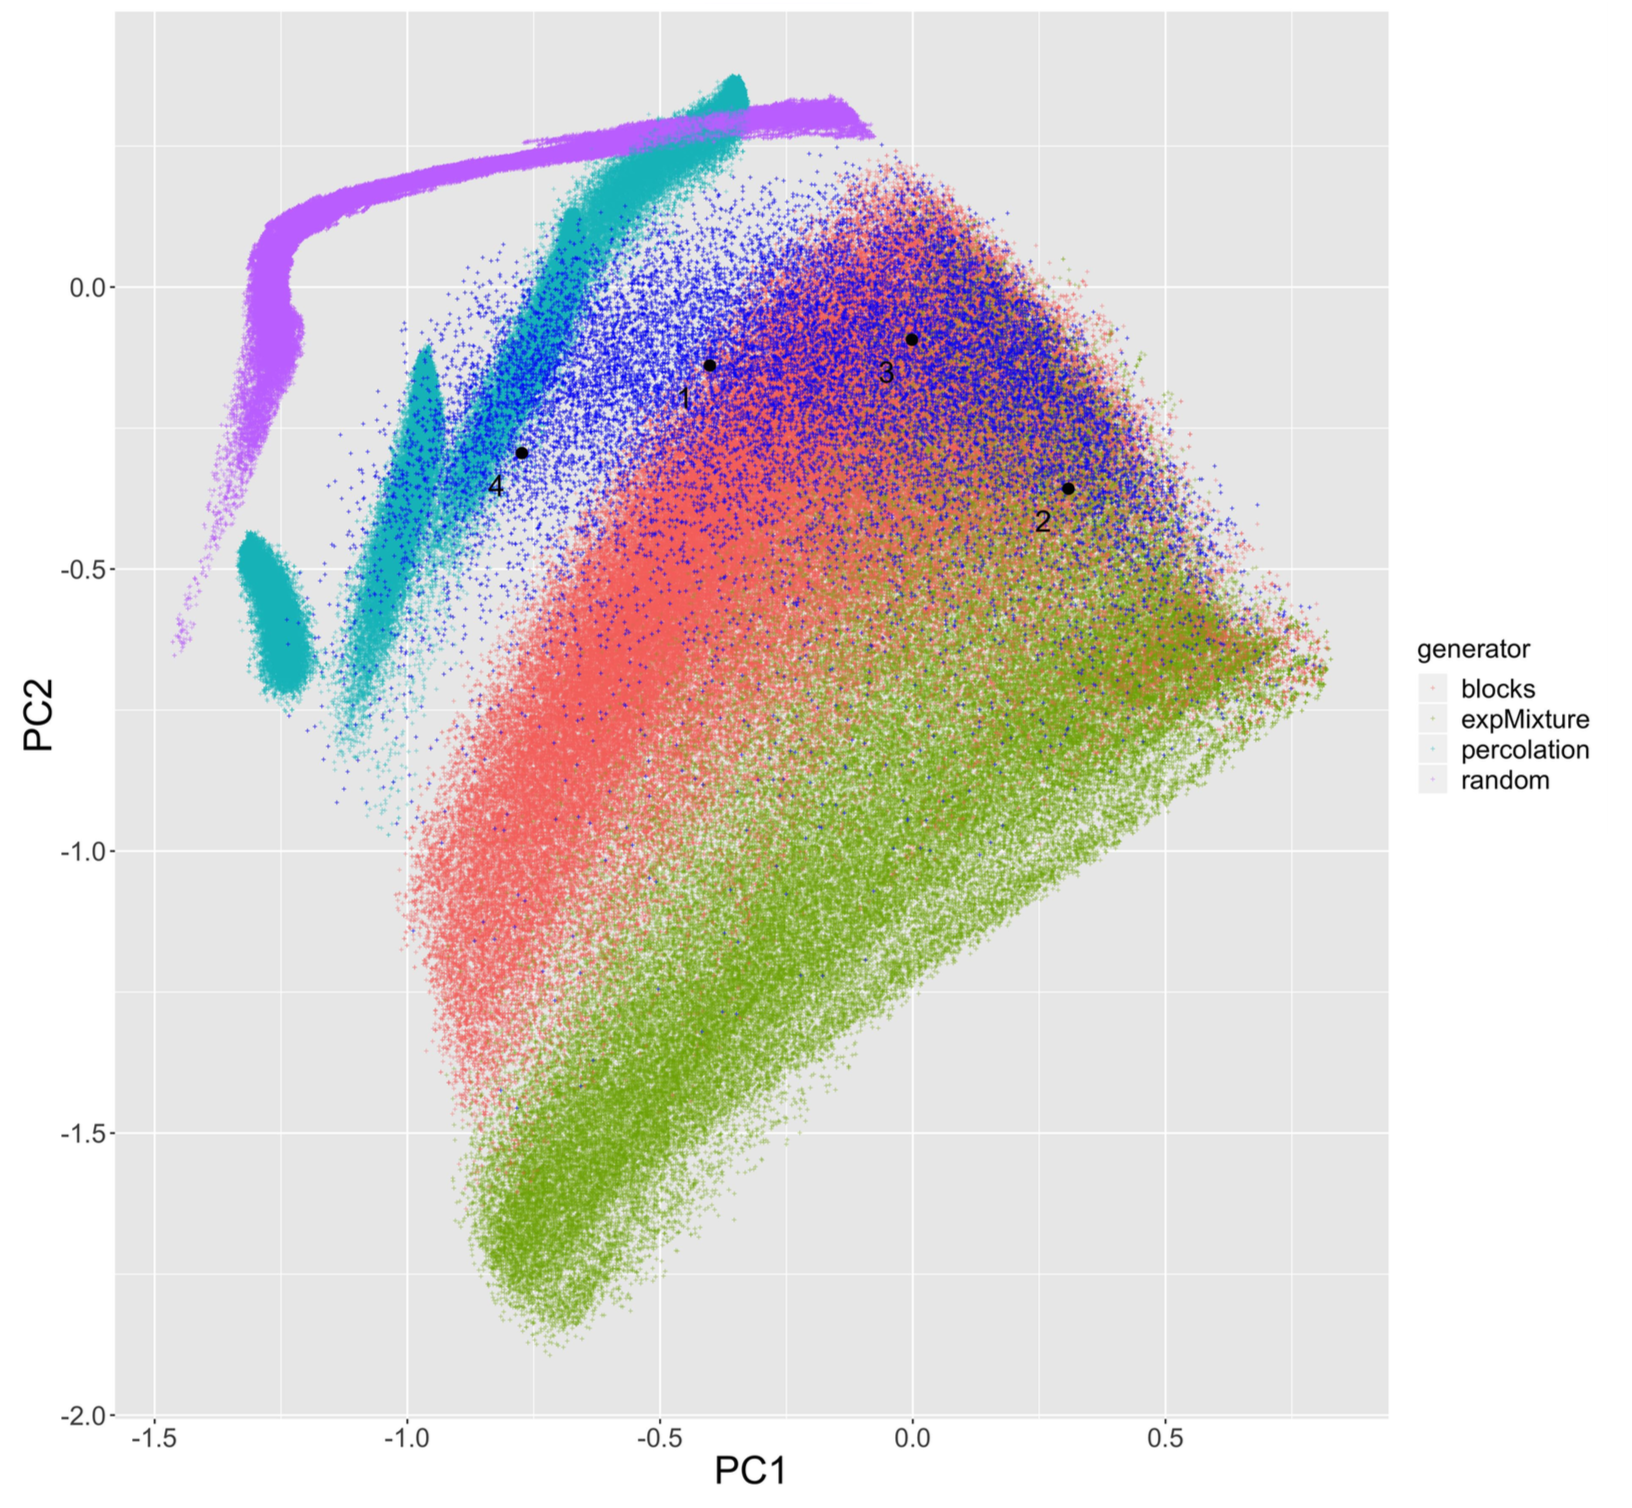
\includegraphics[height=0.8\textheight]{figuresslides/spatialsens_points.png}
\end{center}

\smallskip

\vspace{-0.3cm}
\footnotesize

\textit{Projection of simulated and real cloud points in the real PC space}

}


\sframe{Calibration on classification centroids}{

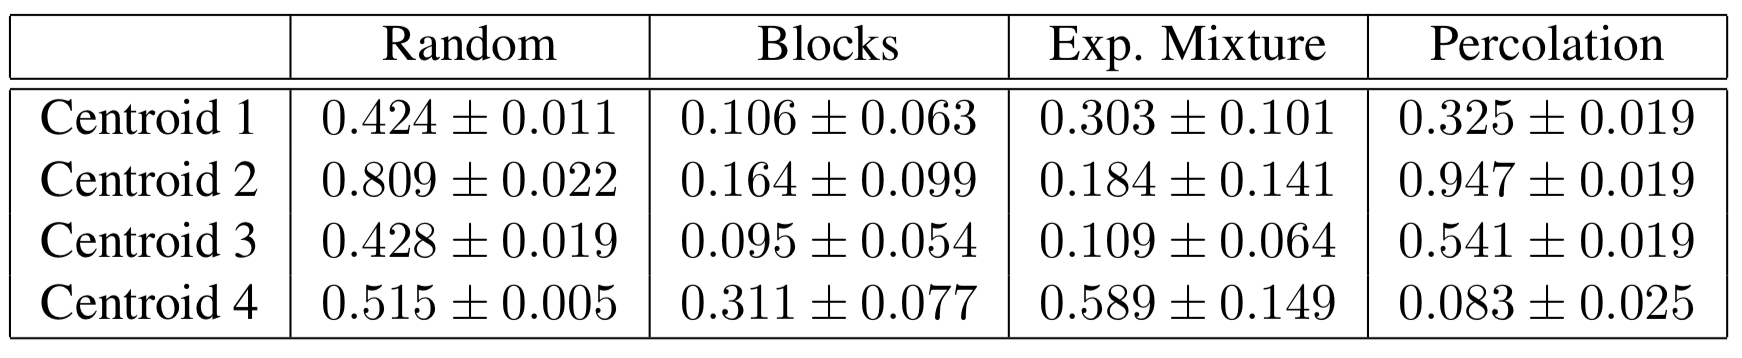
\includegraphics[width=\textwidth]{figuresslides/spatialsens_distanceclasses.png}

\medskip

\textit{Euclidian distances in the projected space, aggregated on stochastic repetitions, for each class centroid and each generator}

%\textit{Why not use calibration heuristics? Open question of fitting a point cloud; issue of projecting in a reduced dimension space}

}


\sframe{Discussion}{

%Our approach provides a first step towards systematic modeling of generative processes of urban form at large scales. Some direct limitations could be tackled in a short term. Testing slightly different processes and heuristics in generator may be a way to cover the part of the real point cloud which is missed by our generators. As it seems correspond to complicated urban centers, it may be however complicated without more elaborated models. Also, we did not use minimization algorithms to calibrate the generators, and the and a further step would consist in checking the robustness of our result using such optimization heuristics (genetic algorithms for example), but also diversity algorithms such as pattern space exploration proposed by \cite{10.1371/journal.pone.0138212}, to ensure the effective feasible space of each generator. 
%This work can also be extended in several ways. First of all, we focused on the built environment but neglected transportation infrastructures, whereas spatial network morphogenesis models have been proposed for example by \cite{courtat2011mathematics} or \cite{raimbault2018multi} in a multi-modeling approach.
%Taking into account multiple dimensions of the urban system is an important extension and hybrid models such as co-evolution models \citep{raimbault2014hybrid} should be investigated.
%\added{Our approach can also be a preliminary step towards the study of urban sustainability issues, for example the relations between urban form and energy consumption }\citep{le2015forme}.\added{ Extending the generators with the third dimension, i.e. taking into account building heights as done by }\cite{brasebin2017apports}\added{, could also be an important component for the study of local energy efficiency.}
%Furthermore, we tested the complementarity of generators only in a static way. Adaptive and dynamic generators, combining processes of different nature within the same model with an endogenous switching or combination, would be an important direction to better understand urban morphogenesis.
%In the same context, the generators compared here had all the same number of parameters, but richer generators implying different numbers would require the use of information criterions to avoid overfitting, which, however, remains an unsolved issue for such generative simulation models \citep{piou2009proposing}.
%Finally, as extensively reviewed above, the way to quantify urban form strongly depends on the scale considered. A more integrative understanding of it would require multi-scale approaches able to relate these different definition and measures within a single multi-scalar framework.

\justify

\vspace{-1cm}

\textbf{Extensions}

\medskip

$\rightarrow$ Apply more elaborated calibration procedures and e.g. diversity search.

\smallskip

$\rightarrow$ Dynamical calibration (issue of sparsity of dynamical urban data).

\smallskip

$\rightarrow$ Take into account possible varying generator parameter number (compensate for overfitting in simulation models \cite{piou2009proposing}).

\bigskip
\bigskip

\textbf{Applications}

\medskip

$\rightarrow$ Link between urban form and sustainability measures: towards insights from generative models.

\smallskip

$\rightarrow$ Towards multi-scale and multi-dimensional models.

\smallskip

$\rightarrow$ Hybridation with more operational approaches \cite{brasebin2017apports}.


}


\sframe{Conclusion}{

% We have proposed here a new insight into the generative simulation of urban morphologies at large scales, namely the scale of the district considering the layout of buildings. After computing morphological measures on a large sample of real urban areas, we showed the complementarity of different generators capturing various aspects of urban morphogenesis processes. Despite not implying generative agents (developers, inhabitants, companies) and thus staying close to procedural modeling, this work however paves the way towards a more systematic understanding of generative processes of urban form at this scale.

\justify
\vspace{-1cm}

$\rightarrow$ New set of urban morphological measures at large scales.

\medskip

$\rightarrow$ Simple generative models with complementary processes to reproduce existing European urban forms regarding morphological indicators.

\medskip

$\rightarrow$ Towards more elaborated models of urban morphogenesis.

\bigskip
\bigskip
\bigskip

\textbf{Code and results available at }\\
\url{https://github.com/openmole/spatialdata}

\bigskip

\textbf{Download OpenMOLE at }\\
\url{https://openmole.org}
 

}





%%%%%%%%%%%%%%%%%%%%%
\begin{frame}[allowframebreaks]
\frametitle{References}
\bibliographystyle{apalike}
\bibliography{biblio}
\end{frame}
%%%%%%%%%%%%%%%%%%%%%%%%%%%%






\end{document}


